\documentclass[tikz, border=10pt]{standalone}
\usepackage{pgfplots}
\pgfplotsset{compat=1.18}
\usetikzlibrary{arrows.meta, decorations.markings, calc}

\begin{document}
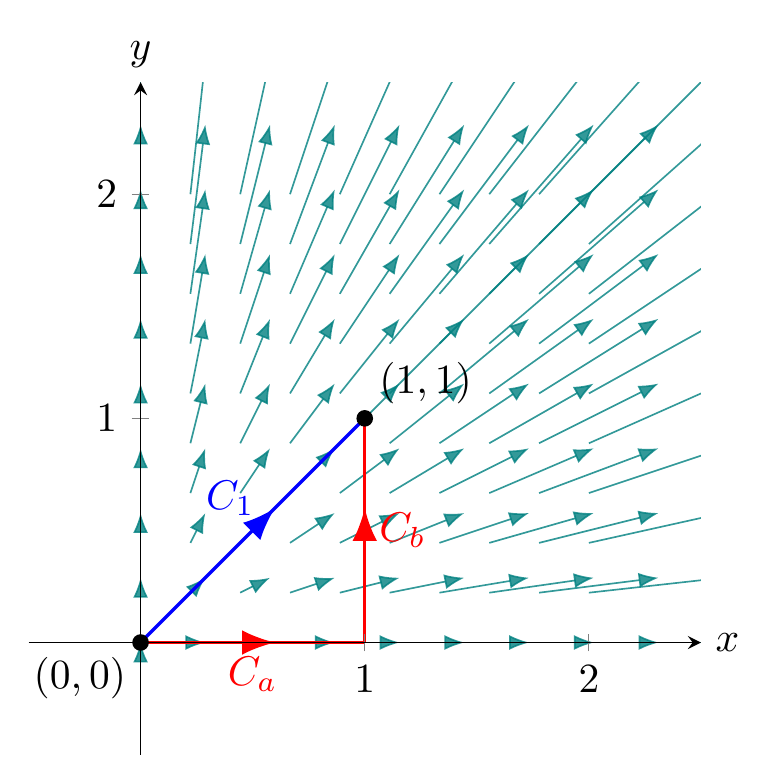
\begin{tikzpicture}[
	scale=1.5,
	% Style for path decorations (arrows in the middle)
	mid arrow/.style={
		postaction={decorate, decoration={
				markings,
				mark=at position 0.6 with {\arrow{Latex[scale=1.2]}}
		}}
	}
	]
	
	\begin{axis}[
		view={0}{90},       % Top-down 2D view
		axis lines=middle,
		xmin=-0.5, xmax=2.5,
		ymin=-0.5, ymax=2.5,
		xlabel=$x$, ylabel=$y$,
		xlabel style={right},
		ylabel style={above},
		zmin=0, zmax=10,    % Arbitrary z-range for clean 2D projection
%		title={\textbf{Conservative Field} $\vec{F} = \langle 2x, 2y \rangle = \nabla(x^2+y^2)$},
		axis equal image,   % Keep aspect ratio 1:1
		grid=major,
		grid style={dashed, gray!30}
		]
		
		% 1. POTENTIAL FUNCTION CONTOURS (f = x^2 + y^2)
		% These are circles centered at origin.
%		% The vector field is always perpendicular to these lines.
%		\foreach \r in {0.5, 1.0, 1.414, 2.0} {
%			\addplot[domain=0:90, samples=40, smooth, thin, gray] ({\r*cos(x)}, {\r*sin(x)});
%		}
%		\node[gray, font=\scriptsize] at (axis cs: 0.2, 1.35) {Contours of $f$};
		
		% 2. THE VECTOR FIELD \vec{F} = <2x, 2y>
		\addplot3[
		quiver={
			u={2*x},    % x-component
			v={2*y},    % y-component
			scale arrows=0.15,
			every arrow/.append style={-Latex, teal, opacity=0.8}
		},
		domain=0:2,
		y domain=0:2,
		samples=10, 
		samples y=10,
		] {0};
		
		% 3. PATH 1: Direct Line (Blue)
		% Parametrization: r(t) = <t, t>
		\addplot[thick, blue, mid arrow] coordinates {(0,0) (1,1)};
		\node[blue, above] at (axis cs: 0.4, 0.5) {$C_1$};
		
		% 4. PATH 2: Stair Step (Red)
		% Step 1: (0,0) -> (1,0)
		\addplot[thick, red, mid arrow] coordinates {(0,0) (1,0)};
		% Step 2: (1,0) -> (1,1)
		\addplot[thick, red, mid arrow] coordinates {(1,0) (1,1)};
		\node[red, below] at (axis cs: 0.5, 0) {$C_{a}$};
		\node[red, right] at (axis cs: 1, 0.5) {$C_{b}$};
		
		% 5. POINTS
		\fill[black] (axis cs: 0,0) circle(2pt) node[below left] {$(0,0)$};
		\fill[black] (axis cs: 1,1) circle(2pt) node[above right] {$(1,1)$};
		
	\end{axis}
\end{tikzpicture}
\end{document}